\section{Introduzione}
\label{sec:capitolo}
\vspace{0.4 em}
\begin{flushleft}
La necessità di digitalizzazione all’interno di aziende o nella pubblica amministrazione, si scontra con la burocrazia “cartacea” ancora molto presente in queste realtà.\\ 
L’idea di questo progetto web nasce proprio dalla possibilità di rendere digitale anche dei piccoli e semplici processi che vengono ripetuti giornalmente all’interno di alcuni uffici che si occupano di ricevere il pubblico. \\
Inizialmente viene proposta all'utente un'autenticazione tramite Google, implementata con OAuth2, il protocollo di rete di tiplogia “access delegation" che consente l'accesso all'applicazione tramite API di sicurezza.\\ 
Questa applicazione web consente di tenere traccia degli ingressi del pubblico in un ufficio attraverso l'inserimento di informazioni tramite un form apposito, in particolare dati relativi alla persona, orario di ingresso, motivazioni della visita.\\ 
I dati inseriti sono memorizzati in un database NoSQL (Not Only SQL), non relazionale, implementato con MongoDB e sono trasmessi in formato JSON (JavaScript Object Notation), utilizzato come alternativa ad XML .\\
In caso di necessità vi è la possibilità di richiedere assistenza all'amministratore del sistema attraverso un Help Desk composto da un form contente le informazioni del richiedente, il messaggio da trasmettere ed un tasto di invio per l’inoltro automatico di email.\\
Inoltre l’amministratore del sistema, per essere informato sulla situazione generale del suo ufficio, a fine giornata, riceverà un riepilogo via email del numerico delle persone che hanno effettuato l’ingresso e le loro indicazioni basilari.\\
Queste informazioni sono fornite tramite query effettuate sul database ed inserite come oggetto delle email di riepilogo.\\
L'importanza dell’aggiornamento del dipendente che accoglie il pubblico sulle ultime notizie, è soddisfatta tramite l'implementazione di una “sezione notizie" nella Home Page, le quali consentiranno una vista globale delle ultime notizie reperibili dal web tramite una ricerca per argomenti di interesse.
\end{flushleft}
 


\newpage
\section{Aspetti tecnologici}
\label{sec:capitolo}
\vspace{0.4 em}
\begin{flushleft}
Gli aspetti tecnologici per questo progetto web si basano sull’utilizzo di API REST per offrire i vari servizi: autenticazione, news, salvataggio dati e query in MongoDB ed invio di email. \\
\subsection{API REST}
Le Application Program Interface operanti all'interno dell'architettura sono di tipo REST (REpresentation State Transfer).\\
Le API REST rispettano l'architettura client/server gestendo le richieste di risorse tramite HTTP e fornendo un'uniformità di interfaccia per i vari componenti, attori del servizio.\\
La rappresentazione delle risorse può essere facilmente manipolata ed utilizzata dal client in quanto fornita tramite JSON, formato altamente leggibile e molto diffuso.\\

\subsection{Autenticazione}
L'implementazione del servizio di autenticazione per l'applicazione, si è reso necessario per garantire l'opportuna sicurezza all'accesso dei dati e delle funzionalità.\\
Modulo fondamentale per il corretto funzionamento della funzionalità è PassportJS, middleware di autenticazione per Node.js.\\
Esso fornisce le c.d. “Strategies" ideate appositamente per servizi di autenticazione come Google, utilizzato in questa applicazione.\\
Essendo un progetto dedicato ed ideato per un utilizzo interno ad un'amministrazione si esige l'aderenza ai requisiti di sicurezza, quali confidenzialità, integrità e disponibilità dei dati (CIA triad). 
\subsubsection{OAuth2 e Google}

L'autenticazione si basa sull'utilizzo di OAuth2. \\
OAuth2 è un protocollo di rete progettato per essere utilizzato con HTTP (Hyper Text Transfer Protocol) ed è considerato lo standard per l'autorizzazione all'accesso ed allo scambio sicuro di dati per servizi web come la Web Application, descritta in questo progetto.\\
Di seguito si riporta il codice delle pagine di authentication.
\lstinputlisting[linerange={ 2-45}]{./settings/code/server.js}

\begin{lstlisting}
\end{lstlisting}
Si riporta successivamente il codice di “auth.js"\\
Si fa presente che il .[dot]env richiamato nella prima riga del codice, è un file di testo di configurazione contenente variabili da passare al sistema.\\
In questo caso contiene il Client ID e il Client Secret fornito dal servizio di Google Credentials per abilitare la autenticazione.\\
\lstinputlisting{./settings/code/auth.js}

\begin{lstlisting}
\end{lstlisting}

\subsection{NewsApi}
Per fornire al dipendente utilizzatore del servizio, una semplice gestione delle informazioni dalle maggiori testate giornalistiche del Paese, i dati vengono richiesti attraverso NewsApi.\\
L’utente ha la possibilità di inserire in uno spazio di ricerca, il tema sul quale vuole ricevere un elenco di notizie.\\
Una volta effettuato l’invio, entra in gioco l’esecuzione dello script news.js, il quale legge l’input, lo utilizza per generare il link per NewsApi ed inoltra la richiesta.\\
La response viene fornita in formato JSON. A sua volta vengono creati i tag html necessari alla visualizzazione in pagina principale del risultato della ricerca..\\
In totale viene mostrato a video un elenco di 20 notizie per argomento ricercato, sotto forma di link.\\
\lstinputlisting{./settings/code/news.js}

\begin{lstlisting}
\end{lstlisting}

\subsection{Database NoSQL MongoDB}
La funzione principale della web app, è devoluta all’inserimento di dati tramite form, ed inviati tramite connessione con il database MongoDB e la libreria Mongoose.\\

\subsubsection{Struttura del database}
Il Database individuato per questa applicazione web è MongoDB. \\
È un database NoSQL (Not Only SQL), caratterizzato dall’essere non relazionale, distribuito, in quanto consente di distribuire su più nodi lo storage ed infine scalabile.
MongoDB è un document database che sfrutta il formato JSON per le query sui dati memorizzati in esso.
La connessione avviene tramite il tool di modellazione degli oggetti “Moongoose” sulla porta 27017, standard per il database e precedentemente definita:

\begin{lstlisting}
mongoose.connect('mongodb://localhost:27017/mydb');
\end{lstlisting}
\vspace{0.4 em}
\newpage
In questo progetto il “document”, in formato JSON, ha una forma del tipo:

\begin{lstlisting}
{
    "_id": {
        "$oid": "abc123"
    },
    "nome": "Francesco",
    "cognome": "Avantaggiato",
    "phone": "123456789",
    "data": "2022-01-01",
    "ora": "23:20",
    "motivazione": "Cambio CI"
	}

\end{lstlisting}
\vspace{0.6em}
Si riporta di seguito la parte di codice estratta da “server.js".\\
In questi passaggi viene anzitutto inizializzata la connessione al database NoSQL, ovvero senza modello relazionale, successivamente viene definita la struttura dello schema.\\
In caso di corretto inserimento dei dati, si reindirizza l'utente ad una nuova schermata, riportante la buona riuscita dell'operazione, nella quale si richiede la successiva attività da intraprendere.\\
\lstinputlisting[linerange={ 105-144}]{./settings/code/server.js}

\begin{lstlisting}
\end{lstlisting}

\subsubsection{Query}
Le query sottoposte al database vengono gestite attraverso la composizione di vari valori di richiesta, utilizzando variabili e funzioni di JavaScript.\\
Di seguito si riporta il codice relativo alle query, con output in console.
\lstinputlisting[linerange={ 157-178}]{./settings/code/server.js}

\begin{lstlisting}
\end{lstlisting}
\newpage

\subsection{Servizio Email - NodeMailer, NodeCron, Mailtrap}

Il servizio di invio email si suddivide in due diverse implementazioni:
\begin{enumerate}
\item invio di email tramite il form dell’Help Desk;
\item invio di email automatico con resoconto giornaliero per l’amministratore.
\end{enumerate}


\subsubsection{Gestione dell'Help Desk}
Il form dell’Help Desk consente all’utente di inviare una mail con una richiesta di assistenza o altre tipologie di richieste, tramite un campo “messaggio” libero.\\
Il funzionamento si basa sull’utilizzo di NodeMailer, un modulo NodeJS che consente il settaggio e l’invio di email, il framework Express, progettato per la creazione di Web Application e di API.\\
Infine un servizio di email sandbox, che consente la creazione di server SMTP fake al solo scopo di development, chiamato MailTrap.\\
Lato server (server.js), viene definita la connessione al servizio tramite porta 2525, l’autenticazione a MailTrap, tramite credenziali fornite dallo stesso e le opzioni email, ovvero la struttura del corpo del messaggio da inviare.\\
Si implementano anche vari console.log e alert per determinare il successo o meno delle connessioni e/o invii di email.\\
Lo script “app.js" consente di prelevare i dati forniti in input ed inviarli tramite AJAX con l’oggetto XMLHttpRequest.\\
XMLHTTP è un set di API che possono essere usate da JavaScript per trasferire XML o altri dati da e verso un web server tramite HTTP.\\
In caso di invio andato a buon fine, vengono ripuliti i campi relativi del form, consentendo eventualmente di effettuare un nuovo inserimento.\\
Si riporta di seguito il codice relativo a quanto descritto.\\
Di seguito il codice.\\
\vspace{0.6 em}
\lstinputlisting[linerange={ 56-94}]{./settings/code/server.js}
\begin{lstlisting}
\end{lstlisting}
\subsubsection{Automatismo dell'invio}
L'invio automatico di mail all'amministratore di sistema basa il suo funzionamento sulle query al database e sull'utilizzo, fondamentale, del modulo Nodecron, il quale consente di settare orari predefiniti e scadenze per l'attuazione di determinate azioni.
In questo caso l'azione è l'invio della mail di resoconto giornaliero, che viene inoltrata nell'orario corrispondente alla chiusura dell'ufficio. \\
Questa impostazione risulta essere a disposizione delle necessità implementative in  ``real life".\\
\lstinputlisting{./settings/code/app.js}
\begin{lstlisting}
\end{lstlisting}
\end{flushleft}
\section{Schema di funzionamento dell'applicazione}
{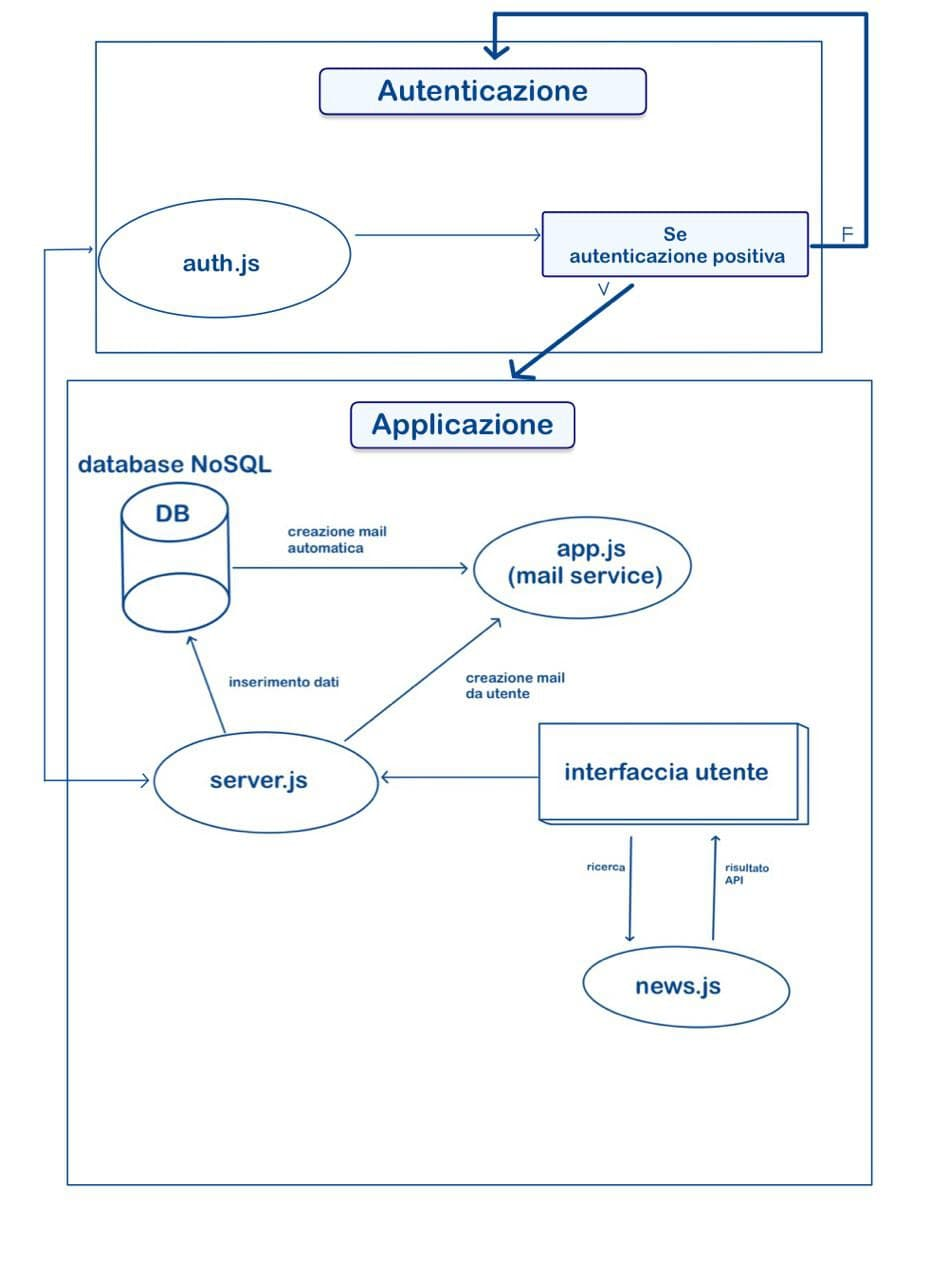
\includegraphics[width= 0.7 \textwidth]{img/schema.jpg}}\\
\newpage
\section{Conclusioni}
\begin{flushleft}


L'architettura della web application messa a disposizione per una variegata tipologia di clientela, si offre all'immediatezza, semplicità e scalabilità.\\
La scelta implementativa dei servizi descritti, si è basata sulla attuale modernità dei frameworks e sull'aderenza del progetto al programma di studio relativo all'insegnamento di Software Oriented Architecture, soprattutto riguardo le API REST.\\
Nella progettazione di questo sito web, si è posta l'attenzione sulle principali problematicità, facendo particolare riferimento all’interazione con l’utente finale.\\
L'importanza dell'autenticazione rappresenta il core principale del servizio, senza la quale esso si presenta come privo di fondamenti di sicurezza per un'architettura da mettere in funzione in tempi moderni.\\
L’utilizzo di query specifiche sul DB, per avere come risultato dati singoli e composti su ciò che è stato fornito in input, è risultato essere determinante per l’implementazione di alcune funzioni successive come quella dell’invio automatico di email.\\
Si è posta attenzione alla figura dell’amministratore in quanto utente principale,identificato come referente nel caso di ricorso all’Help Desk ed individuo in grado di ricevere aggiornamenti costanti sulla situazione generale del servizio, con resoconti inviati tramite testo di una email.

\section{Note Sitografiche}
\begin{enumerate}

\item W3school \url{https://www.w3schools.com/}\\
\item OAuth - documentation \url{https://oauth.net/}\\
\item PassPortJS - documentation https://www.passportjs.org/docs/
\item Google APIs - credentials \url{https://console.cloud.google.com/apis/credentials}\\
\item MongoDB - documentation \url{https://docs.mongodb.com/}\\
\item MailTrap Guide \url{https://mailtrap.io/}\\
\item Nodemailer - documentation \url{https://nodemailer.com}\\
   
\end{enumerate}
\end{flushleft}